\documentclass[border=8pt]{standalone}
\usepackage{mathpazo}
\usepackage{tikz}
\usepackage{pgfplots}
\pgfplotsset{compat=1.18}

\definecolor{stblue}{HTML}{7B97AD}
\definecolor{rwgold}{HTML}{B8995E}
\definecolor{sage}{HTML}{7A9A7E}
\definecolor{terracotta}{HTML}{C47A6A}
\definecolor{dkbrown}{HTML}{3D3530}
\definecolor{wmgray}{HTML}{7B7067}
\definecolor{rosewood}{HTML}{AD8480}

\begin{document}
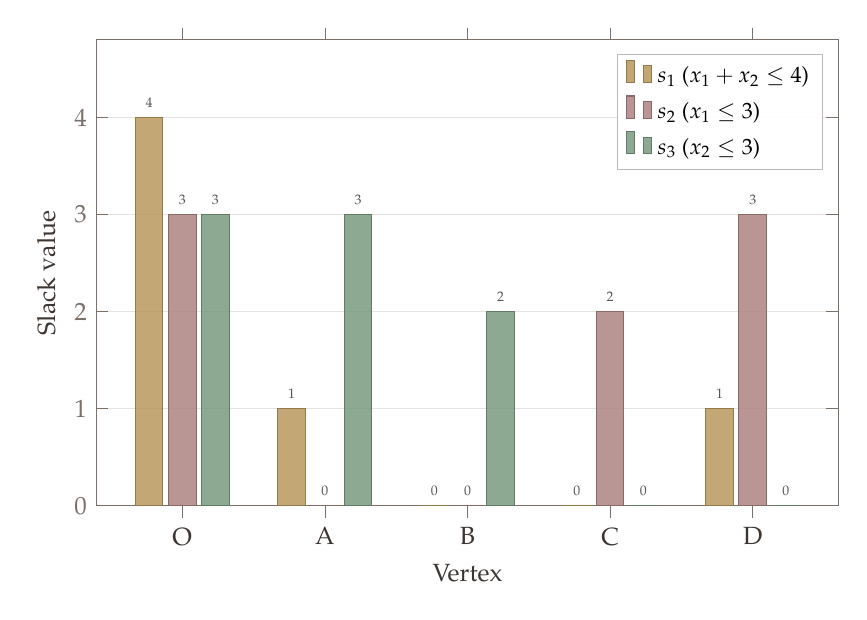
\begin{tikzpicture}
\begin{axis}[
    ybar,
    bar width=10pt,
    width=11cm,
    height=7.5cm,
    enlarge x limits=0.15,
    ylabel={Slack value},
    ylabel style={font=\small,dkbrown},
    xlabel style={font=\small,dkbrown},
    symbolic x coords={O,A,B,C,D},
    xtick=data,
    xticklabel style={font=\small,dkbrown},
    yticklabel style={font=\small,wmgray},
    ymin=0,
    ymax=4.8,
    ytick={0,1,2,3,4},
    legend style={
      at={(0.98,0.97)},
      anchor=north east,
      font=\footnotesize,
      draw=wmgray!50,
      fill=white,
      fill opacity=0.9,
      text opacity=1,
      row sep=1pt,
    },
    legend cell align={left},
    axis line style={wmgray},
    tick style={wmgray},
    major grid style={wmgray!20},
    ymajorgrids=true,
    xlabel={Vertex},
    every node near coord/.append style={font=\tiny,dkbrown},
    nodes near coords,
    nodes near coords align={vertical},
    every axis plot/.append style={fill opacity=0.85},
]
\addplot[fill=rwgold,draw=rwgold!80!black] coordinates {(O,4) (A,1) (B,0) (C,0) (D,1)};
\addplot[fill=rosewood,draw=rosewood!80!black] coordinates {(O,3) (A,0) (B,0) (C,2) (D,3)};
\addplot[fill=sage,draw=sage!80!black] coordinates {(O,3) (A,3) (B,2) (C,0) (D,0)};
\legend{$s_1$ ($x_1+x_2 \leq 4$),$s_2$ ($x_1 \leq 3$),$s_3$ ($x_2 \leq 3$)}
\end{axis}
\end{tikzpicture}
\end{document}
